\documentclass[11pt]{article}

\usepackage[letterpaper,margin=0.75in]{geometry}
\usepackage{booktabs}
\usepackage{graphicx}
\usepackage{listings}
\usepackage{hyperref}

\setlength{\parindent}{1.4em}

\begin{document}

\lstset{
  language=Python,
  basicstyle=\small,          % print whole listing small
  keywordstyle=\bfseries,
  identifierstyle=,           % nothing happens
  commentstyle=,              % white comments
  stringstyle=\ttfamily,      % typewriter type for strings
  showstringspaces=false,     % no special string spaces
  numbers=left,
  numberstyle=\tiny,
  numbersep=5pt,
  frame=tb,
}

\newenvironment{absolutelynopagebreak}
  {\par\nobreak\vfil\penalty0\vfilneg
   \vtop\bgroup}
  {\par\xdef\tpd{\the\prevdepth}\egroup
   \prevdepth=\tpd}

\title{Network Simulation}

\author{Cody Heffner}

\date{22 Jan. 2015}

\maketitle

\section{Preface}

This report details the experiment I ran and the results obtained as specified by the Reliable Transport Lab in the BYU CS 460 class taught by Dr. Zappala. The project specifications can be found \href{http://cs460.byu.edu/winter-2015/labs/reliable-transport}{here}.

The experiment requires heavy use of a network simulator to test different network scenarios. The network simulator I used is Dr. Zappala's \href{https://github.com/zappala/bene}{Bene}, written in Python. All my simulation examples shown will be tailored towards use for that simulator.

\section{Summary}

The goal of the experiment was to show that reliable transport of data is possible and that dynamic retransmission timers work and are effective. The first section of the report describes how I implemented reliable transport. The second section discusses my implementation of a dynamic retransmission timer and includes data and analysis of my implementation.

\section{Reliable Transport}

Reliable transport in TCP is simply achieved by the sender marking each segment with the number of the starting byte of data. In other words, if the sender is sending bytes 30-50, the sender marks the segment with the value \emph{30}. When the receiver receives a segment, it replies with the value of the next byte it expects to receive. When the sender receives bytes 30-50 (after already obtaining bytes 1-29), it replies with a value of \emph{51} because that is the next byte it doesn't have yet. 

By coding this behavior into my TCP implementation, I was able to acheive reliable transport and send files in a variety of unreliable networks. The following blocks show my experimental data in 10 Mbps networks with propagation delays of 10 ms, varying window sizes, varying files, and varying loss rates. The files used were all obtained from Zappala's Bene repository.

\vspace{0.5cm}
\begin{absolutelynopagebreak}
\begin{tabular}{lcc}
  \toprule
  Window Size & Loss Rates & File Name & Transfer Time\\
  \midrule
  3000 & 00\% & test.txt & 0.088 s\\
  3000 & 10\% & test.txt & 2.1064 s\\
  3000 & 20\% & test.txt & 4.1064 s\\
  3000 & 50\% & test.txt & 34.1664 s\\

  10,000 & 00\% & internet-architecture.pdf & 1.451616 s\\
  10,000 & 10\% & internet-architecture.pdf & 49.361216 s\\
  10,000 & 20\% & internet-architecture.pdf & 88.019616 s\\
  10,000 & 50\% & internet-architecture.pdf & 420.112643 s\\
  \bottomrule
\end{tabular}
\end{absolutelynopagebreak}
\vspace{0.5cm}

All outputs received the message \"File transfer correct!\" as the last line, indicating that all bytes were received. For implementation details and code discussion, please see Appendix A.

\section{Dynamic Retransmission Timer}

\vspace{0.5cm}
\begin{absolutelynopagebreak}
\begin{tabular}{lcc}
  \toprule
  Window Size & Loss Rates & File Name & Transfer Time\\
  \midrule
  3000 & 00\% & test.txt & 0.088 s\\
  3000 & 10\% & test.txt & 0.757262 s\\
  3000 & 20\% & test.txt & 2.479328 s\\
  3000 & 50\% & test.txt & 10.68372 s\\

  10,000 & 00\% & internet-architecture.pdf & 1.451616 s\\
  10,000 & 10\% & internet-architecture.pdf & 26.480791 s\\
  10,000 & 20\% & internet-architecture.pdf & 46.874493 s\\
  10,000 & 50\% & internet-architecture.pdf & 395.76971 s\\
  \bottomrule
\end{tabular}
\end{absolutelynopagebreak}
\vspace{0.5cm}

\section{Appendix A: Reliable Transfer Code}

The following section shows my TCP methods relevant to reliable transfer. They rely heavily on the \emph{buffer} class implemented by Dr. Zappala in the Bene simulator.

\vspace{5mm}
\begin{absolutelynopagebreak}
\begin{lstlisting}
''' Sender '''

def send(self,data):
    ''' Send data on the connection. Called by the application. '''
    self.send_buffer.put(data)
    while self.send_buffer.available() > 0 and self.send_buffer.outstanding() < self.window:
        if self.send_buffer.outstanding() + self.mss > self.window:
            (seg_data,i) = self.send_buffer.get(self.window - self.send_buffer.outstanding())
        else:
            (seg_data,i) = self.send_buffer.get(self.mss)
        self.send_packet(seg_data,i)

def send_packet(self,data,sequence):
    packet = TCPPacket(source_address=self.source_address,
                       source_port=self.source_port,
                       destination_address=self.destination_address,
                       destination_port=self.destination_port,
                       body=data,
                       sequence=sequence,ack_number=self.ack)

    # send the packet
    self.trace("%s (%d) sending TCP segment to %d for %d" % (self.node.hostname,self.source_address,self.destination_address,packet.sequence))
    self.transport.send_packet(packet)

    # set a timer
    if not self.timer:
        self.timer = Sim.scheduler.add(delay=self.rtt, event='retransmit', handler=self.retransmit)
    
    # record when it was sent
    self.add_to_timer(sequence)

def handle_ack(self,packet):
    ''' Handle an incoming ACK. '''
    self.trace("%s (%d) Incoming ACK received from %d for %d" % (self.node.hostname, packet.destination_address, packet.source_address, packet.ack_number))
    self.sequence = packet.ack_number
    self.send_buffer.slide(packet.ack_number)
    self.recalculate_timeout(packet.sequence)
    if self.send_buffer.outstanding() == 0:
        self.cancel_timer()
        self.send("")
    else:
        self.restart_timer()

def retransmit(self,event):
    ''' Retransmit data. '''
    self.trace("%s (%d) retransmission timer fired" % (self.node.hostname,self.source_address))
    self.timer = Sim.scheduler.add(delay=self.timeout, event='retransmit', handler=self.retransmit)
    (data, i) = self.send_buffer.resend(1000)
    self.send_packet(data, i)
    self.remove_from_timer(i)
\end{lstlisting}
\end{absolutelynopagebreak}

As can be seen from the code, the sender is handed data in the \emph{send} function and immediately puts it in the buffer. It then retrieves data from the buffer no greater than the maximum segment size and continues to send that data using the \emph{send_packet} function until the buffer tells it to stop. The \emph{send_packet} function simply sends the segment to the transport layer. The \emph{handle_ack} method manages the buffer and timer book-keeping. Finally, the \emph{retransmit} function is called when a timer expires; it sends a single packet to the receiver because it hasn't heard back from the receiver in time.

===========================================================

\section{Three Nodes}

For the three-node portion of the experiment, I set up three separate networks. The following list enumerates the three scenarios for which I needed separate networks. 

\begin{enumerate}

\item Two Fast Links, Part A: In a network consisting of three nodes A, B, and C, perform the transfer of a 1 MB file divided into 1000 1 kB packets from node A to C. The links include a link from A to B with 100 ms propagation delay and 1 Mbps bandwidth, and a link from B to C otherwise identical to the first link.

\item Two Fast Links, Part B: In a network consisting of three nodes A, B, and C, perform the transfer of a 1 MB file divided into 1000 1 kB packets from node A to C. The links include a link from A to B with 100 ms propagation delay and 1 Gbps bandwidth, and a link from B to C otherwise identical to the first link.

\item One Fast Link and One Slow Link: In a network consisting of three nodes A, B, and C, perform the transfer of a 1 MB file divided into 1000 1 kB packets from node A to C. The links include a link from A to B with 100 ms propagation delay and 1 Mbps bandwidth, and a link from B to C with 100 ms propagation delay and 256 Kbps bandwidth.

\end{enumerate}

By inspection, all these scenarios are nearly identical. I will only show the raw code for the first network. The following two code blocks show the .txt file describing the network to Bene and the Python file that executes the experiment.

\vspace{5mm}
\begin{absolutelynopagebreak}
\begin{lstlisting}
# 3n1a.txt
    # n1 -- n2 -- n3
    #
    n1 n2
    n2 n1 n3
    n3 n2

    # link configuration
    n1 n2 1Mbps 100ms
    n2 n1 1Mbps 100ms
    n2 n3 1Mbps 100ms
    n3 n2 1Mbps 100ms
\end{lstlisting}
\end{absolutelynopagebreak}

\vspace{5mm}

\begin{absolutelynopagebreak}
\begin{lstlisting}
# sim.py
    # setup network
    net = Network('networks/3n1a.txt')

    # setup routes
    n1 = net.get_node('n1')
    n2 = net.get_node('n2')
    n3 = net.get_node('n3')
    n1.add_forwarding_entry(address=n2.get_address('n1'),link=n1.links[0])
    n1.add_forwarding_entry(address=n3.get_address('n2'),link=n1.links[0])
    n2.add_forwarding_entry(address=n1.get_address('n2'),link=n2.links[0])
    n2.add_forwarding_entry(address=n3.get_address('n2'),link=n2.links[1])
    n3.add_forwarding_entry(address=n2.get_address('n3'),link=n3.links[0])
    n3.add_forwarding_entry(address=n1.get_address('n2'),link=n3.links[0])

    # setup app
    d = DelayHandler()
    net.nodes['n1'].add_protocol(protocol="delay",handler=d)
    net.nodes['n2'].add_protocol(protocol="delay",handler=d)
    net.nodes['n3'].add_protocol(protocol="delay",handler=d)
\end{lstlisting}
\end{absolutelynopagebreak}
\vspace{5mm}

Upon close inspection of sim.py, the network needs to be set up in a slightly different way than the two-node network. This network needed six different forwarding table entries compared with two entries in the two-node network. This is because there needs to be a forwarding table entry from \emph{each} node to \emph{every other} node. As you can see from the code, a forwarding table entry is added from n1 to n2 and to n3, then from n2 to n1 and to n3, then finally from n3 to n2 and to n1. The most interesting cases are from n1 to n3 and back. N1 doesn't have a direct link to n3, so it must go through n2. Thus, the forwarding table entry from n1 to n3 needs to specify that it needs to go to the address n3 has dedicated to receive from n2, and it needs to run on the first (and only) link n1 has - the link to n2. Beyond that, it is up to the implementation of the node class to know how to differentiate packets that have arrived at their destination and need to be forwarded.

In the first scenario of transferring a 1 MB file across a pretty fast network, the simulation calculated that the file transfer was complete at time t=8.208s. For the second scenario of transferring a 1 MB file across a very fast network, the simulation calculated that the file transfer was complete at time t=0.208008s. The unbalanced network scenario, where one link was fast and one link was slow, resulted in a file transfer time of t=31.458s.

\vspace{0.5cm}
\begin{absolutelynopagebreak}
\begin{tabular}{lcc}
  \toprule
  Scenario & File Transfer Time\\
  \midrule
  1 & 8.208s \\
  2 & 0.208008s \\
  3 & 31.458s \\
  \bottomrule
\end{tabular}
\end{absolutelynopagebreak}
\vspace{0.5cm}

These values correlate exactly with the answers I calculated in the first homework assignment. The equation used to calculate the delay of the first scenario with a pretty fast network is:

\vspace{5mm}
\begin{absolutelynopagebreak}
\begin{lstlisting}
t = (2*transmission + 2*propagation) + 999 * transmission
  = (2*(8000 bits / 1000000 bps) + 0.200s) + 999 * (8000 bits / 1000000 bps))
  = (0.216s) + 999 * 0.008s
t = 8.208s
\end{lstlisting}
\end{absolutelynopagebreak}
\vspace{5mm}

In this scenario, the first bit of the first packet is set on the line from n1 to n2 at t=0s. It travels to n2 in one \emph{propagation} delay length of time, arriving at n1 at t=100ms. It sits and waits at n2 for the trailing bits to arrive, which takes one duration of the \emph{transmission} delay. When the whole packet has arrived at n2, the first bit is sent on the line to n3 immediately, because there is no other packet ahead of it. It arrives at n3 in one more \emph{propagation} length of time (accounting for \emph{2*propagation} in the formula above), then must wait one more \emph{transmission} length of time (accounting for \emph{2*transmission} in the formula above). When the first packet is at n3, all other packets will be streaming in back-to-back at n3. The file transfer will be complete when n3 has received 999 more packets, all taking a duration equal to the \emph{transmission} delay to arrive.

In the second scenario, the same formula may be used as long as corrections are made to the transmission delay. The transmission delay in this scenario is 1000 times smaller because the link is 1000 times faster while the packet size and number of packets are equivalent. The only delay that doesn't shrink is the propagation delay - this stays the same as the first scenario.

In the third scenario, a new variable is introduced: the queueing delay. Because the second link has lower bandwidth, n2 will not be able to transmit packets as fast as it receives them. N2 will need to store incoming packets in a queue so that it will not lose packets if it's still busy transmitting other packets to n3. I derived the formula to calculate the queueing delay in my homework and will not re-derive it here. The following block shows the basic formula representing this scenario as well as the calculated answer, which is equal to the value received by the simulator.

\vspace{5mm}
\begin{absolutelynopagebreak}
\begin{lstlisting}
queue(n) = L(K-1)(1/Rslow - 1/Rfast)
t = 1000 * transfast + prop + queue(1000) + 1000 * transslow + prop
  = 1000 * 0.008s + 0.1s + 23.226750s + 1000 * 0.03125s + 0.1s
t = 31.458s
\end{lstlisting}
\end{absolutelynopagebreak}
\vspace{5mm}

\section{Queueing Theory}

The final part of my experiment was to validate queueing theory for an M/D/1 queue. An M/D/1 queue is a single queue that receives packets as an exponential distribution and services those packets deterministically. The following enumeration describes my process for this part of the experiment. The corresponding code is shown below the enumeration. 

\begin{enumerate}

\item I modified some existing code in Bene's \emph{delay.py} script. The only modifications I made were to run the simulation for a longer duration and to allow me to vary the utilization of the server's queue directly from the command line. The goal of this code is to throw packets at the node at random times, rather than predetermined like in previous experiments.

\item Next, I created a parser to average the queue time of each packet from \emph{delay.py}'s output. 

\item I then created a shell script to run all the simulations at once. 

\item Finally, I created a Python script to graph my results compared with the theoretical expected behavior.

\end{enumerate}

\vspace{5mm}
\begin{absolutelynopagebreak}
\begin{lstlisting}
# delay.py
    #arguments
    parser = argparse.ArgumentParser(prog='Delayed Packets')
    parser.add_argument('-u', '--util', type=float, action='store', default='all')
    args = parser.parse_args()
    utilization = args.util

    # parameters
    Sim.scheduler.reset()

    # setup network
    net = Network('../networks/one-hop.txt')

    # setup routes
    n1 = net.get_node('n1')
    n2 = net.get_node('n2')
    n1.add_forwarding_entry(address=n2.get_address('n1'),link=n1.links[0])
    n2.add_forwarding_entry(address=n1.get_address('n2'),link=n2.links[0])

    # setup app
    d = DelayHandler()
    net.nodes['n2'].add_protocol(protocol="delay",handler=d)

    # setup packet generator
    destination = n2.get_address('n1')
    max_rate = 1000000/(1000*8)

    load = utilization*max_rate
    g = Generator(node=n1,destination=destination,load=load,duration=1000)
    Sim.scheduler.add(delay=0, event='generate', handler=g.handle)
    
    # run the simulation
    Sim.scheduler.run()
\end{lstlisting}
\end{absolutelynopagebreak}

\vspace{5mm}

\begin{absolutelynopagebreak}
\begin{lstlisting}
# delayparser.py
    class Delayparser(object):
        def __init__(self):
            pass

        def parse(self, filename):
            f = open(filename, "r")

            avg = 0.0
            count = 0.0
            # skip the first line
            for line in f.readlines():
                if (line[0] != 'R' and line[0] != '\n'):
                    avg += float(line.split(' ')[6].split('\n')[0])
                    count += 1
            return [count, avg / count]

    if __name__ == '__main__':
        d = Delayparser()

        util = [10, 20, 30, 40, 50, 60, 70, 80, 90, 95, 98]

        for u in util:
            f = "outputs/qt_" + str(u) + ".txt"
            ret = d.parse(f)
            print "{:.0f}% utilization: {:.0f} packets, {:.6f} average queue delay.".format(u, ret[0], ret[1])
\end{lstlisting}
\end{absolutelynopagebreak}

\vspace{5mm}

\begin{absolutelynopagebreak}
\begin{lstlisting}
# delay.sh
    python delay.py -u 0.1 >> outputs/qt_10.txt
    python delay.py -u 0.2 >> outputs/qt_20.txt
    python delay.py -u 0.3 >> outputs/qt_30.txt
    python delay.py -u 0.4 >> outputs/qt_40.txt
    python delay.py -u 0.5 >> outputs/qt_50.txt
    python delay.py -u 0.6 >> outputs/qt_60.txt
    python delay.py -u 0.7 >> outputs/qt_70.txt
    python delay.py -u 0.8 >> outputs/qt_80.txt
    python delay.py -u 0.9 >> outputs/qt_90.txt
    python delay.py -u 0.95 >> outputs/qt_95.txt
    python delay.py -u 0.98 >> outputs/qt_98.txt

    python delayparser.py > outputs/average_queueing_delay.txt
\end{lstlisting}
\end{absolutelynopagebreak}

\vspace{5mm}

\begin{absolutelynopagebreak}
\begin{lstlisting}
# plot.py
    # Class that parses a file and plots several graphs
    class Plotter:
        def __init__(self):
            self.x = [0.1, 0.2, 0.3, 0.4, 0.5, 0.6, 0.7, 0.8, 0.9, 0.95, 0.98]
            self.y = [0.000463, 0.001016, 0.001702, 0.002650, 0.003899, 0.006066, 0.009240, 0.016074, 0.032784, 0.081299, 0.205917]

        def combinedPlot(self):
            """ Create a graph that includes a line plot and a boxplot. """
            clf()
            ax = plt.figure().add_subplot(111)

            # plot the data
            plot(self.x, self.y, label='Theory')

            # plot the equation
            # u = 125                           # service rate = 1/transmission delay = R / L
            p = np.arange(0, 0.995, 0.001)      # utilization
            y = []
            for i in range(0, len(p)):
                y.append(1.0/(2.0*125.0) * (p[i])/(1.0-(p[i])))
            plot(p, y, label='Average')

            # set up the axis
            xlabel('Utilization')
            ax.set_xticks(np.arange(0,1.1,0.1))
            ylabel('Average Queue Duration')
            ax.set_yticks(np.arange(0,0.7,0.1))

            # create a legend
            legend = ax.legend(loc='upper left', shadow=True)

            #print it out
            savefig('outputs/lab1_final.png')

    if __name__ == '__main__':
        p = Plotter()
        p.combinedPlot()
\end{lstlisting}
\end{absolutelynopagebreak}
\vspace{5mm}

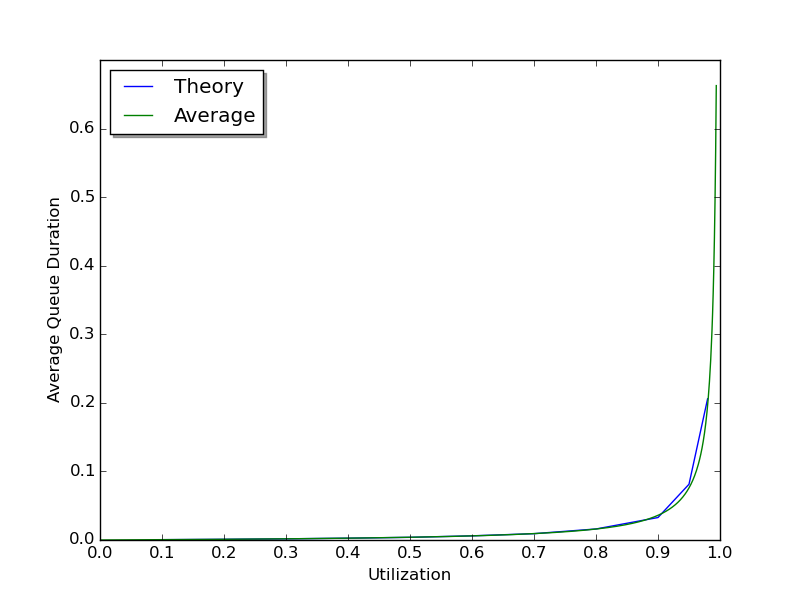
\includegraphics[width=17cm]{outputs/lab1_final.png}

The final result is a graph showing the relationship between the theoretical and actual queueing delay produced by the simulator. The correlation between theory and observed is extremely high. 

\section{Conclusion}

This experiment confirmed the behavior of the internet that we have learned about so far in CS 460 - that is, it confirmed how propagation, transmission, and queueing delays work, and that queueing theory is valid with an M/D/1 queue.

During the queueing theory portion of the experiment I ran into some trouble that gave me deeper insight on how the internet works. I left the duration to throw packets at the server at 10 seconds. This made my data vary \emph{greatly}, to the point where higher utilization levels weren't anywhere near the theoretical curve. I attempted to run this experiment multiple times to get more data points to average. This improved my data slightly but not to the point where I'd feel comfortable saying this experiment verified queueing theory. After looking through the code, I changed the duration from 10 to 100 seconds. This led to significant improvement. I increased it further to 1000 and got the results shown above. 

I pondered why running the experiment multiple times would not improve results but increasing the duration would. I came to the conclusion that by running multiple iterations, I was allowing the server's queue to clear. Just by periodically allowing the server's queue to clear every 10 seconds, the queue time at higher utilizations was reduced more than 50\%.

This could be an interesting area of research for another time: what is the relationship between periodic breaks and queue times at various utilizations? How high can utilization of servers be pushed if they are periodically allowed breaks? Would this be more efficient or effective than keeping utilizations low?

\end{document}
